\section{Balancers}
\label{sec:balancers}
\subsection{Theoretical Preliminaries}
In order to express our load balancing algorithms, we first present the precise load balancing problem and then introduce our model terminology and the trellis load balancing concept.
%Before we can express the manner in which tasks are distributed across the cluster, we must first identify our tasks. 
As mentioned in Section \ref{sec:calibration}, elements are agglomerated into tiles to amortize the scheduling overhead.  The simulation consists of many tasks, each one responsible for advancing a single tile by one RK stage.  Based on the DG kernel \eqref{eq:dgkernel}, any edge between two elements on different tiles constitutes a dependency. In order to minimize the number of dependencies and expose the largest amount of asynchrony, we group elements into tiles using the METIS $k$-way graph partitioning algorithm \cite{realmetis}.
%Given enough parallelism, the delay associated with message delivery can be hidden via tile oversubscription.
%Due to the high compute cost associated with the DG kernel compared to network message delivery in our experiments, we've found it sufficient to ensure that there are at least two tiles per worker thread.

%Given this set of tiles, we formulate our load balancing problem.
Each tile $i$ will have a memory space requirement $m_i$, and an amount of work required to advance the tile by one RK stage will be given by $t_i$. We now introduce the assignment variables, $\chi_{ik}$, where
\begin{displaymath}
\chi_{ik} = \begin{cases}
1 & \text{if tile $i$ is on rank $k$}\\
0 & \text{otherwise}
\end{cases},
\end{displaymath}
and $\chi_{ik}$ is subject to the following constraints:
\begin{equation}
\sum_{k=1}^{n_{\text{ranks}}} \chi_{ik} =1 \quad \forall\, i=1,\ldots,n_{\text{tiles}}.
\label{eq:toor}
\end{equation}
Ideally, we would solve for time-dependent values of $\chi_{ik}$ that minimize the total application execution time. However, for asynchronous applications, this is an NP-hard mixed integer optimal scheduling problem, which is not feasible to solve in situ. Since the compute cost of the tiles dominates the execution time, we make the simplifying assumption that the execution time is approximately proportional to 
\begin{equation}
T = \max_k \sum_{i=1}^{n_{\text{tiles}}} t_i \chi_{ik}
\label{eq:extime}
\end{equation}
Additionally, we also have a memory constraint, namely, if $m_i$ is the memory required for tile $i$ and $M_k$ is the available memory on rank $k$, then we obtain the additional constraints:
\begin{equation}
\sum_{i=1}^{n_{\text{tiles}}} m_i \chi_{ik} \le M_k \quad \forall k=1,\ldots,n_{\text{ranks}}.
\label{eq:memconst}
\end{equation}
Our optimization problem is defined by \eqref{eq:toor}, \eqref{eq:extime}, and \eqref{eq:memconst}. Note that since the tile's compute cost changes as the simulation progresses, the optimal assignment $\{\chi_{ik}\}$ is also a function of the simulation's progress.  Furthermore, the irregularity associated with the wetting and drying algorithm requires that the memory constraint \eqref{eq:memconst} and the execution time \eqref{eq:extime} are accounted for separately.
%At any instant during the simulation, the solution can be approximated using the multi-constraint graph partitioning algorithm outlined by Karypis et al. in \cite{KKMC}. 
Before we discuss approaches to approximate optimal assignments $\{\chi_{ik}\}$, we introduce some formalism upon which we will base our load balancing strategies.

\subsubsection{The trellis approach}
The main idea of this approach is to execute a second, parallel task dependency graph to handle load balancing that is completely independent of the application task graph.
The motivation for this approach is twofold: it decouples the load balancer from the application execution, avoiding the need for costly control synchronization and it accurately accounts for the improvement in load balance with the cost of making load balancing decisions.

First, a common strategy taken by semi-static load balancers is to periodically pause application execution, issue data and task migrations (rebalancing phase), and resume application execution.
This strategy is convenient because it decouples the times during which tasks and data are allowed to be in transit from the times that tasks are executing and sending messages to each other.
%, so the locations of data and tasks are fixed and known to all processes during task execution.
Unfortunately, in order to enter and exit the rebalancing phase, control dependencies are added to the application task graph (often in the form of global synchronization), which can severely impact the performance of a highly asynchronous execution model.
The trellis approach introduces an ancillary set of tasks that collect the application state, make rebalancing decisions, and launch tile migrations, all without adding synchronization to the application execution.

Another advantage of the trellis approach is the fixed frequency and natural amortization of the cost of rebalancing.
%, i.e. our load balancer would get less aggressive for more imbalanced applications.
Were the frequency of rebalancing instead linked to application progress, the frequency of rebalancing would {\em decrease} as the load balance {\em worsens} since each iteration would take longer to complete.
Additionally, assuming reasonable strong scaling, doubling the simulation core count would approximately double the frequency of the load balancer even though the cost of the load balancer would remain the same.
In practice, there is a trade-off between the improvement in run-time due to improved load balance and the cost of rebalancing.
%, e.g. resource starvation while tasks wait for the migrating tile to arrive at the new rank and satisfy its dependencies. 
%For our strong scaling example, the doubled frequency would now require a modified cost model, since we've presumably doubled the cost of rebalancing.
%We assume that the performance benefit is dependent on the change in imbalance, and by relating rebalancing frequency to application progress, we've introduced an artificial dependence on the core count into our load balancing frequency.
The trellis approach allows us to simplify our cost model,
% by not having to take the core counts into consideration, 
reducing the numbers of parameters that need to be tuned in order to maintain effective load balancing.

\subsubsection{Local models}

The second bit of formalism we would like to introduce, are \emph{local models}.  
% These models become necessary due to distributed nature of our computations.  
These models capture local states of the system that can be used to make load balancing decisions.
The use of local models reduces the need to aggregate global information; however, it is infeasible to keep all model information up-to-date at all times, thus the information in these models can become stale.  If a rank steals a tile based on stale information, the tile migration could in fact negatively impact the load balance.
Since this information is exclusively used for load balancing, the correctness of the numerical simulation remains unaffected.
For our problem, we consider 3 types of models:
\begin{enumerate}
\item \emph{Tile model}: Information such as the location and compute load of neighboring tiles.
\item \emph{Rank model}: Information such as how much work is located on a rank (may aggregate local tile models).
\item \emph{World model}: Information about the global state of the simulation (may aggregate tile and rank models).
\end{enumerate}
The nested nature of these models is represented in Figure \ref{fig:localmodels}.
These models provide representations of the simulation upon which the load balancers make relocation decisions.
% Additionally, since the tiles are registered in the AGAS, the tile models will follow their respective tiles as they are relocated.  This minimizes unnecessary data creation and deletion and also simplifies rank model data structures.
%Equipped with these tools, we are ready to describe to our load balancing procedures. 

\begin{figure}
  %\vspace{-5mm}
  \centering
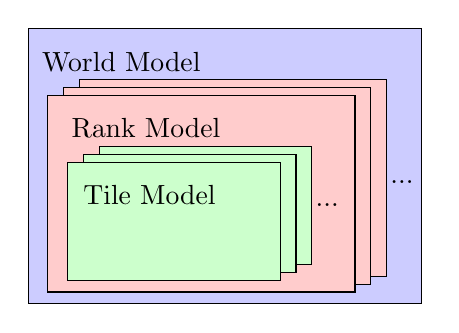
\begin{tikzpicture}
%World Model
\draw [fill=blue!20] (0,1.5) rectangle (5.,5.);
\node[text width=2.25 cm,align=left,below=5pt] at (1.3,5.0) {World Model};
\draw [fill=red!20] (0.65,1.85) rectangle (4.55,4.35);
\draw [fill=red!20] (0.45,1.75) rectangle (4.35,4.25);
\draw [fill=red!20] (0.25,1.65) rectangle (4.15,4.15); %3.5 2.5
\node[text width=0.4 cm] at (4.8, 3.05) {...};
\node[text width=2 cm,align=left,below=5pt] at (1.55,4.15) {Rank Model};
\draw [fill=green!20] (0.9,2.0) rectangle (3.6,3.5);
\draw [fill=green!20] (0.7,1.9) rectangle (3.4,3.4);
\draw [fill=green!20] (0.5,1.8) rectangle (3.2,3.3);
\node[text width=0.4 cm] at (3.85, 2.75) {...};
\node[text width=2 cm, align=left,below=5pt] at (1.7,3.3) {Tile Model};
\end{tikzpicture}
\caption{Each world model is able to aggregate rank models, which aggregate tile models. This allows for representations of the system with various levels of completeness.}
\label{fig:localmodels}
%\vspace{-5mm}
\end{figure}

\subsection{Static load balancing}

%The first attempt at solving the load-balancing problem arises from Seny et al \cite{seny}. 
By re-imagining the wetting and drying algorithm as a type of multirate timestepping, where the dry elements have an infinitely large timestep and the wet elements advance at the implemented timestep, we use the static load balancing approach outlined in \cite{seny}. Here the goal is to assign an equal number of dry elements and wet elements to each rank. This is accomplished by using the multi-constraint graph partitioning outlined in \cite{KKMC}. Note that balancing the memory and load constraints and balancing the wet and dry elements are equivalent formulations of the same load balancing problem.

\subsection{Dynamic load balancing}
Dynamic load balancers in our context are defined as load balancing strategies that operate in an entirely {\em distributed, asynchronous}  manner.
The methods relocate tiles based on a ``load pressure''---the local difference in loads. The idea is to issue many individual relocation requests based on these local observations, and thereby achieve a global balance.

To accommodate both memory and load balance objectives, we implement the refinement procedure used in \cite{KKMC}.
Specifically, our asynchronous diffusion approach includes no world model, but we include tile models and rank models outlined in Listings \ref{lst:tm} and \ref{lst:rm}.


\begin{lstlisting}[
float,
label={lst:tm},
caption={Asynchronous Diffusion Tile Model}]
struct TileModel {
  int my_rank;
  map<int,int> neigh_rank;
  double wet_fraction;  
  double get_gain(int rank);
  void local_broadcast();
};
\end{lstlisting}

\begin{lstlisting}[
float,
label={lst:rm},
caption={Asynchronous Diffusion Rank Model}]
struct RankModel {
  map<int,pair<double,double>> rank_weight;
  StealQ boundary_data;
  void local_broadcast();
  void update_boundary(int leaving);
  void steal_one_tile();
};
\end{lstlisting}

The tile model consists of the tile's wet fraction, the location of neighboring tiles, and a communication gain function, which determines the net impact on inter-rank communication were the tile to be relocated.
The rank model aggregates its tile models to include the tiles bordering the rank, changes in the rank's load balance, and a list of neighboring ranks. These neighboring tiles are stored in the \texttt{StealQ}.
A rank periodically broadcasts its load balancing information to its neighbors,
%Due to the symmetric nature of the communication pattern, 
allowing ranks to aggregate the load state of neighboring ranks.
The execution model does not guarantee message ordering. In order to ensure correctness, both tile and rank models call a \texttt{local\_broadcast} function, which updates neighbors' rank and tile states at regular intervals.
The \texttt{StealQ} contains two STL maps for each rank. This data structure allows us to prioritize, which tile to steal to balance an imbalance in wet or dry tiles from a given rank. The maps are sorted by the amount of extra communication that would be required after stealing a given tile; we prioritize stealing tiles that minimize this additional communication.

During the execution of a task, the tile checks to determine if the wet fraction has switched between wet and dry states.
In the case this happens, the tile's local broadcast updates neighboring tile models.
%, which is then incorporated into the neighbors' rank models.
AGAS {\tt visit} is utilized to ensure that updates are delivered to the tiles no matter where they are located.
The rank model periodically calls \texttt{steal\_one\_tile()}.
Based on the rank model's estimation of the neighboring ranks' work and memory loads, the rank assembles a priority queue $\mathcal{PQ}$ sorted by normalized wet- and dry-element counts.
Only ranks that are overworked or have too many tiles will be inserted into this queue; overburdened ranks will never steal tiles. Karypis and Kumar note this stealing heuristic may lead to chatter, which is when tiles get passed back and forth between the same ranks. To mitigate this, we introduce admissible pressure gradients, i.e. a required minimum imbalance to warrant being inserted into the pool of candidate ranks to be stolen from. Specifically, let the granularity $\mathcal{G}$ be the largest number of elements per tile. For a given rank $r$, let $\mathcal{D}(r)$ be the number of dry elements on rank $r$ and $\mathcal{W}(r)$ the number of wet elements on rank $r$. The precise heuristic for inserting elements is shown in Algorithm \ref{alg:heur}.

\begin{figure}
\begin{algorithm}[H]
\caption{Asynchronous Diffusion Thresholding}
\begin{algorithmic}
\State Set $r$ to current rank ID
\State Set $\Sigma_{\mathcal{W}} \gets \mathcal{W}(r) + \sum_{n \in \text{neighbors}(r)} \mathcal{W}(n)$
\State Set $\Sigma_{\mathcal{D}} \gets \mathcal{D}(r) + \sum_{n \in \text{neighbors}(r)} \mathcal{D}(n)$
\ForAll {$n \in \text{neighbors}(r)$}
    \If {$\mathcal{W}(r) + \alpha \mathcal{G} < \mathcal{W}(n)$}
        \State Insert $n$ into $\mathcal{PQ}(r)$ with weight $\mathcal{W}(n)/\Sigma_{\mathcal{W}}$.
    \EndIf
    \If {$\mathcal{D}(r) + \beta \mathcal{G} < \mathcal{D}(n) $}
        \State Insert $n$ into $\mathcal{PQ}(r)$ with weight $\mathcal{D}(n)/\Sigma_{\mathcal{D}}$.
    \EndIf
\EndFor
\end{algorithmic}
\label{alg:heur}
\end{algorithm}
\end{figure}
Then, we attempt to find the tile on the most imbalanced neighboring rank, which borders the stealing rank and would result in the best communication gain. If there is no satisfactory tile to select, we attempt to improve the most imbalanced constraint associated with the next most-imbalanced rank.

\subsection{Semi-static load balancing}
While the dynamic load balancing procedure allows for fully distributed load balancing decisions, it is unclear that this will result in a good global load balance. The multi-constraint partitioning problem may result in unconnected partitions \cite{KKMC}.  Additionally, the thresholding heuristic is unable to correct gradual--yet large--load imbalances.

To ensure, that we have a good load balance, we consider a semi-static approach which periodically rebalances the global model.  In our formalism, the tile model updates the world model with its wet fraction at a fixed frequency.  Therefore, we can trigger a load balance when all the tiles have sent their information without having to perform any synchronization. %Additionally,
%since we don't begin load balancing until all tile models' messages have been processed, this coordination of broadcast frequency 
%we can minimize the staleness of the tile models by ensuring that all the tiles send their information within a relatively small time interval.
The global model incorporates all the information required to perform load balancing, i.e. the current tile partition and an approximation to the current wet fractions of the respective tiles. The global model is the only entity which may issue {\tt relocate}s, as such the tile partition stored in the global model is always accurate.
%\todo{we removed the more complex algorithm referenced here}

Semistatic rebalancing involves constructing an updated tile-to-rank assignment based on the constraints associated with the updated wet fractions using the multi-constraint graph partitioning algorithm \cite{KKMC}. To keep the master threads available to process messages, we offload the relatively expensive rebalancing operations onto the worker threads where the global model is stored. After obtaining this new partition, we potentially have the means to load balance the system. However, the multi-constraint graph partitioner is unable to take into account the previous location of the tiles. As a worst case scenario, the graph partitioner could return the same partition with permuted partition IDs. The resulting relocation would require migration of every tile, whereas simply maintaining the old partition we would achieve the same load balance without disruption.
In order to remedy this, we solve a minimization problem which determines a permutation in the global rank ID names, which minimizes the number of tiles to be migrated. Using a greedy method, we construct a priority queue of old ID and new ID pairs weighted by the number of tiles that reside in both partitions. We then pop the members of the priority queue until all of the ranks have been assigned new IDs.
This approach can have a significant impact on the number of tiles migrated: for example, during a 1200 core run with 4,400 tiles, the greedy assignment reduced the total number of tiles migrated from roughly 317,000 to 106,000.